\section{Tracking with the Inner Detector} \label{sec:atlas:tracking}

With its closest component, the insertable b-layer (IBL)
\cite{Potamianos:2209070}, only 3.3 cm from the interaction point The Inner
Detector (ID), shown in figure \ref{fig:inner_detector_diagram}
\cite{ATLAS-TDR-4,ATLAS-TDR-5}, faces the incredible challenge of providing
precision momentum resolution and identification of both primary and secondary
vertex measurements of charged tracks all while recieving the highest fluence.

\begin{figure}[!htbp]
  \begin{center}
    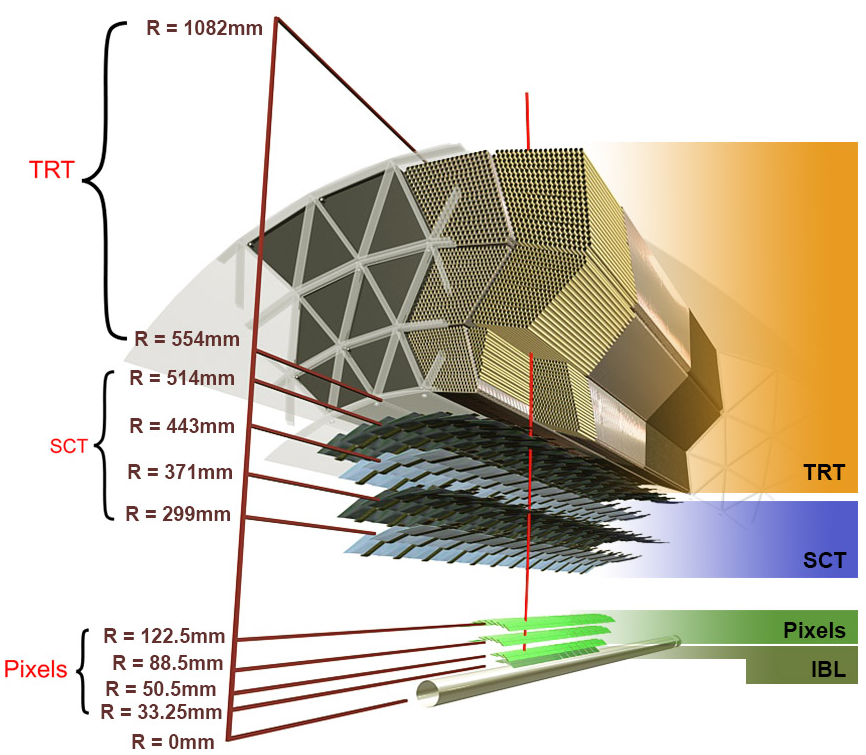
\includegraphics[width=0.8\linewidth]{figures/atlas/inner_detector_diagram}
    \caption{ \cite{Potamianos:2209070} Diagram of inner detector}
    \label{fig:inner_detector_diagram}
  \end{center}
\end{figure}

It is designed to be very compact to reduce the probability of a particle
decaying inside and to give precision measurements of the particles curvature in
the 2T solenoidal magnetic field. This leades to excellent momentum resolution
above the nominal \pT threshold of $0.5$GeV and within the pseudorapidity range
of $|\eta| < 2.5$ as shown in figure \ref{fig:inner_detector_schematic}

\begin{figure}[!htbp]
  \begin{center}
    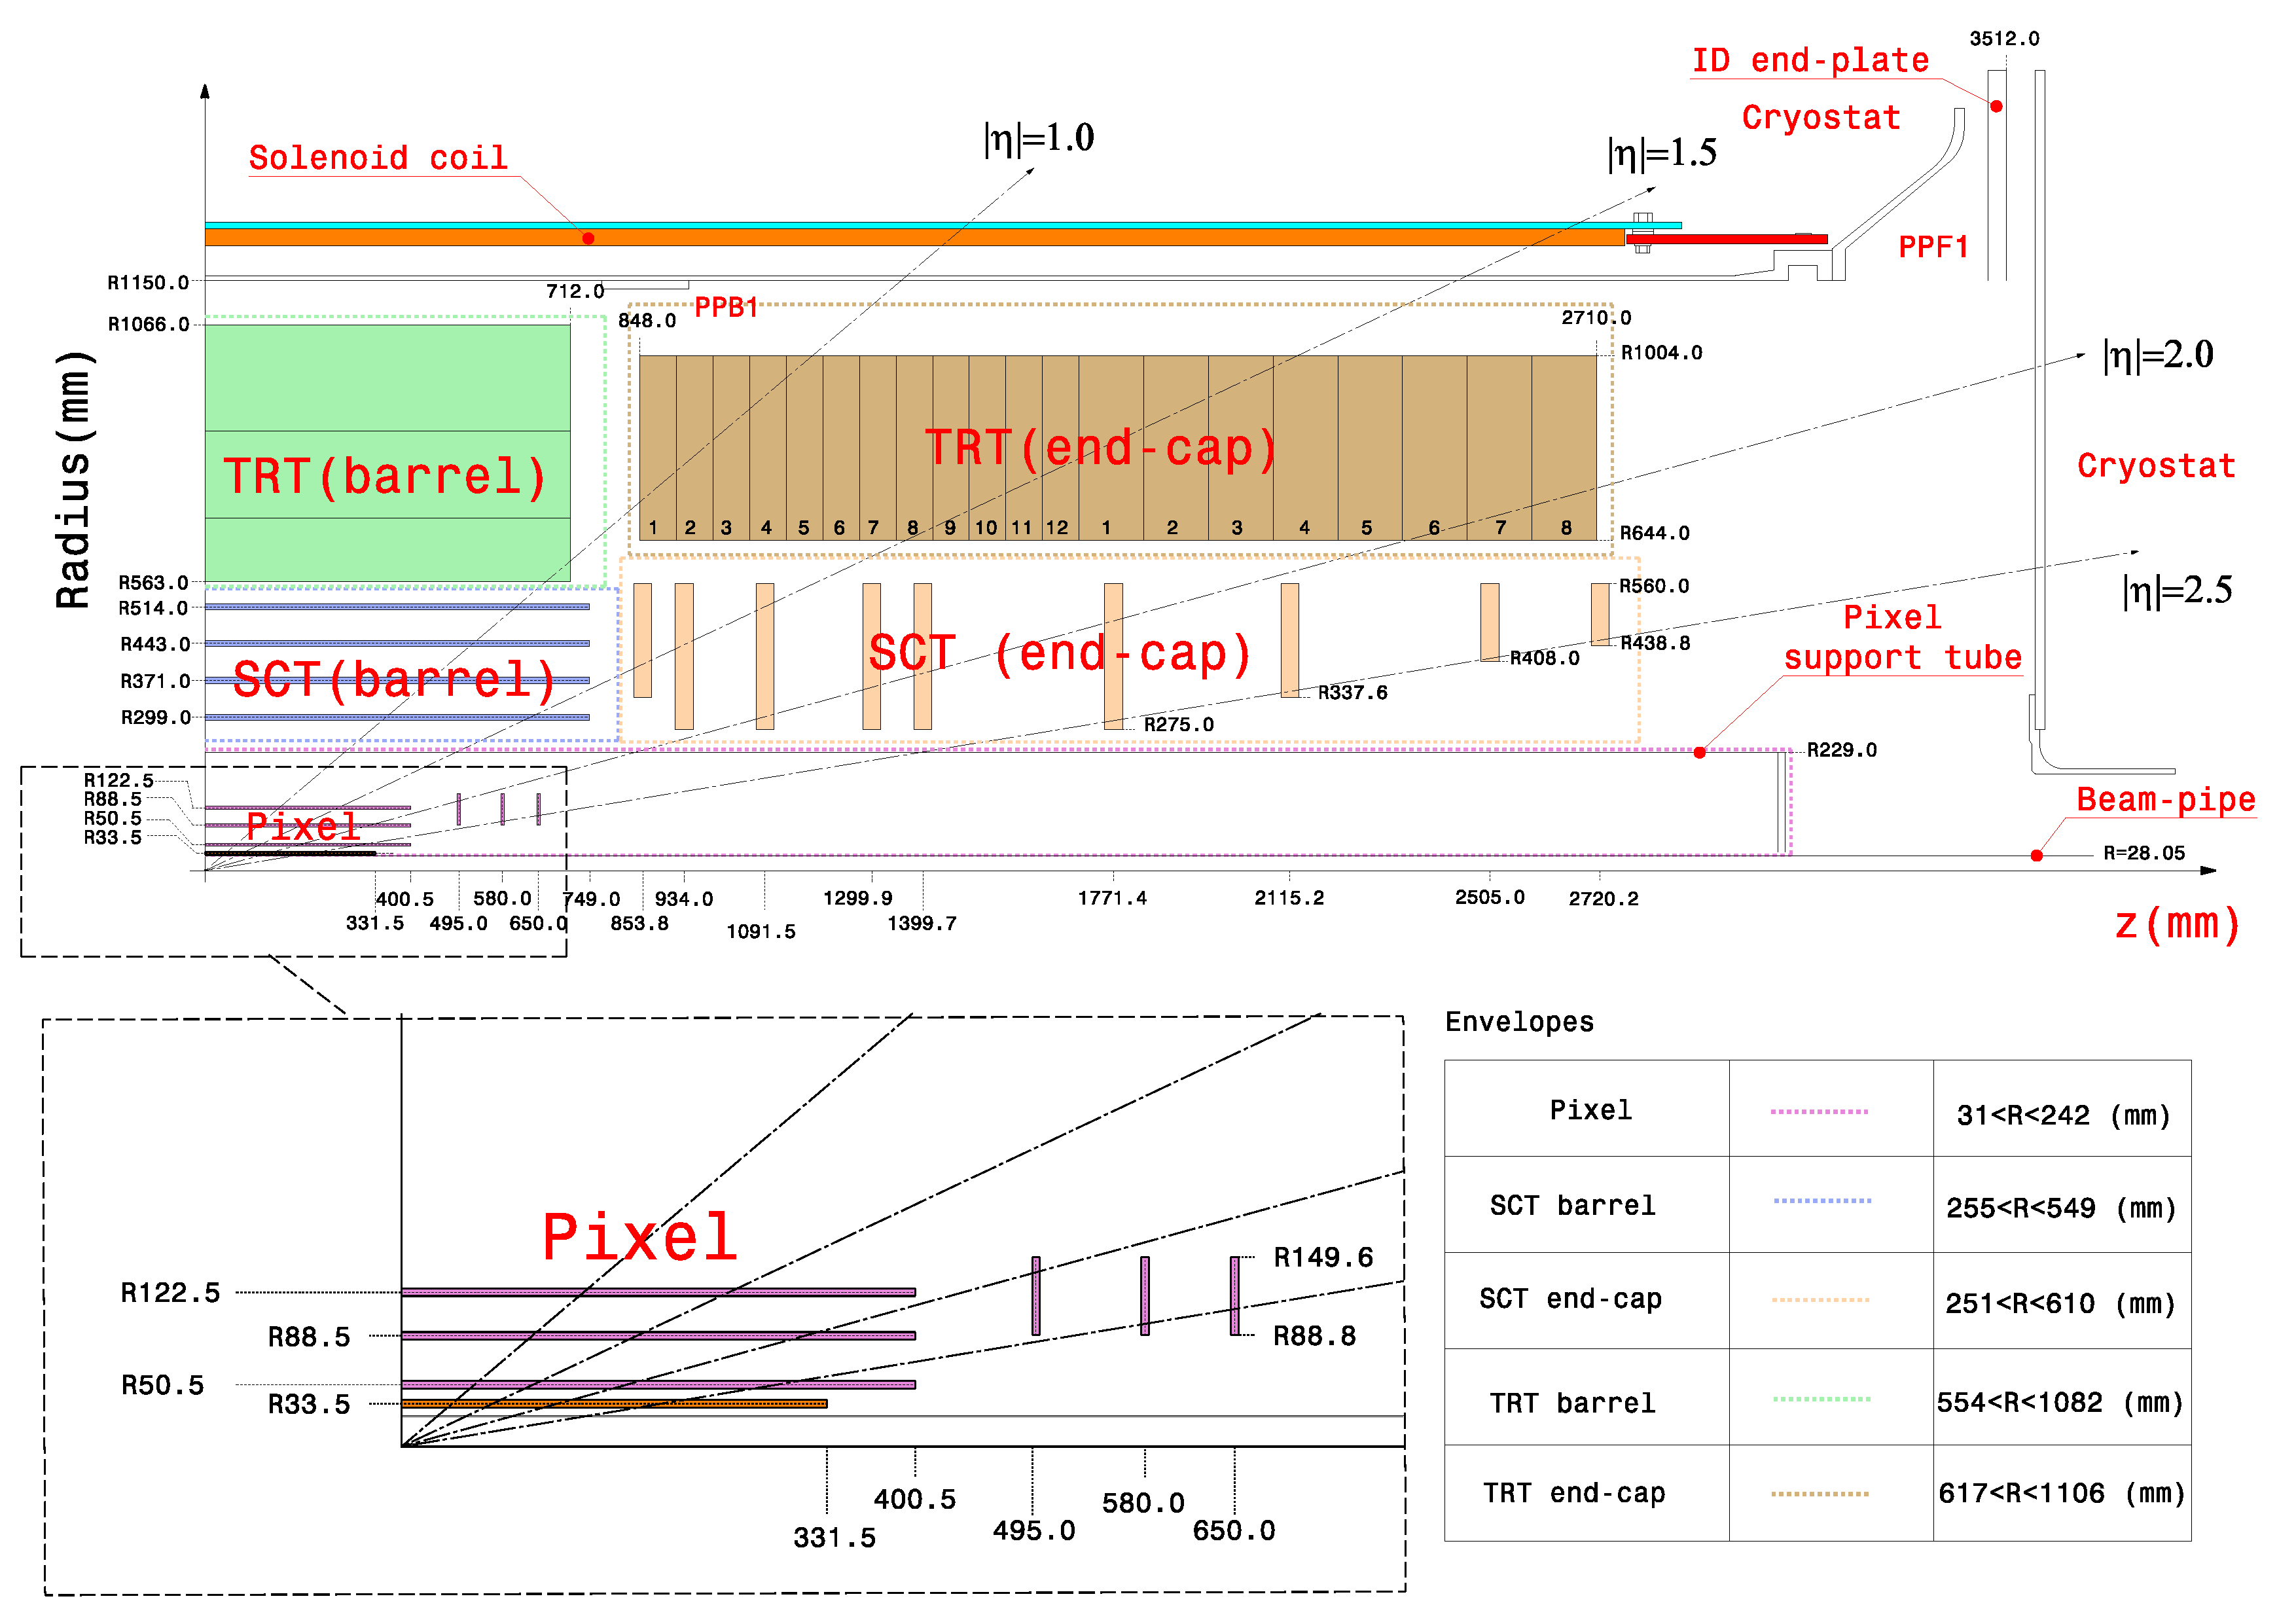
\includegraphics[width=0.8\linewidth]{figures/atlas/inner_detector_schematic}
    \caption{ \cite{PIX-2018-001} Schematic of the Inner Detector including eta
lines.  Each component shown is cylindrically symmetric leading to a
multi-layered detector.}
    \label{fig:inner_detector_schematic}
  \end{center}
\end{figure}

The ID is composed of three different detector technologies for particle
trajector reconstruction: The Pixel Detector, Semiconductor Tracker (SCT) and
the Transition Radiation Tracker (TRT).  These will be discussed in the
following sections. 

\subsection{Pixel Detector}

The ATLAS Pixel Detector, the innermost subdetector of the ID, is designed to
give the best resolution possible as close as possible to the interaction point.
This is accomplished using the 4 barrel layers and the 3 disks per endcap as
indicated in figure \ref{fig:inner_detector_schematic}. The inner most barrel
layer, the IBL, has pixel dimensions of $50\mu $m$(\hat{\phi}) \times 250\mu $m$
(\hat{z}) \times 200\mu $m$(\hat{r})$.  For the other layers the dimensions are
$50\mu $m$(\hat{\phi}) \times 400\mu $m$(\hat{z})$ for about $90\%$ of the pixels
and $50\mu $m$(\hat{\phi}) \times 600\mu $m$(\hat{z})$ for the others, all with a
thickness of $250\mu $m$(\hat{r})$.  This gives a total active area of $1.88 $m$^2$
collected through 92.4 million readout channels, more than half of the total
number of channels for ATLAS. This detailed charged particle information very
close to the interaction point is crucial not only for pattern recognition for
track reconstruction, but also for the reconstruction of the primary and
secondary verticies intrinsic to the decay of a $b$-hadrons, a critical element
of the analysis presented in this thesis.

\subsection{Semiconductor Tracker}

Encompassing the Pixel Detector, the Semiconductor Tracker (SCT) is composed of
double sided silicon microstrips modules.  Each side of the 4088 modules
contains 768 active strips each one $12.6$cm long, alligned with $\hat{z}$ in
the barrel and $\hat{r}$ in the end caps, and separated by a $80 \mu$m pitch
width in the $\hat{\phi}$ direction. The two sides are rotated with respect to
eachother by $40 \mu$m to allow for position measurement in the $z$ direction.
These modules are then used to tile the 4 barrel layers and 9 disks per endcap
(18 disks in total) as seen in figure \ref{fig:inner_detector_schematic}.  This
design is choosen to ensure that each charged track interacts with 8 strip
layers (4 module assemblies).  This information is used to further measure the
momentum, impact parameter, and vertex identification of charged particles.

\subsection{Transition Radiation Tracker}





